\documentclass[../main.tex]{subfiles}
\graphicspath{{\subfix{../figures/}}}

\begin{document}
\section{开放封闭原则(OCP)}
Open Close Principle

软件应该是可扩展,而不可修改的。也就是说,对扩展是开放的,而对修改是封闭的。

\textbf{Meyer 开闭原则}:Bertrand Meyer在1988年提出,一个实体(类、函数)类的实现只应该因错误而修改,新的或者改变的特性应该通过新建不同的类实现。
\begin{figure}[H]
  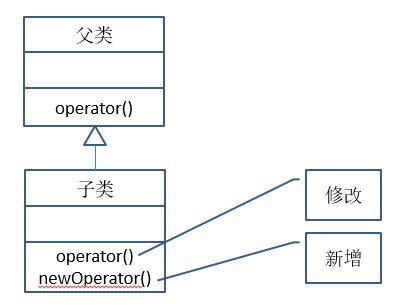
\includegraphics[width=0.35\textwidth]{9_1.jpg}
  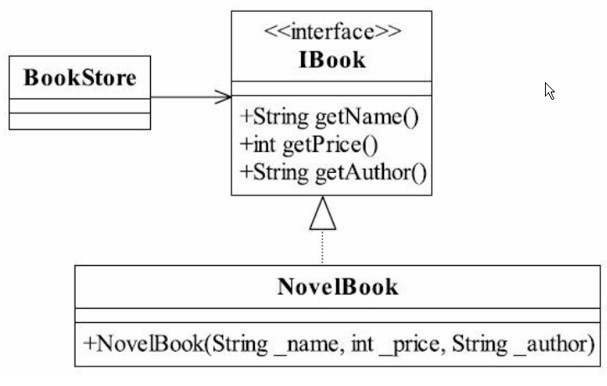
\includegraphics[width=0.45\textwidth]{9_2.jpg}
\end{figure}
\textbf{遵循 OCP 带来的好处}:
\begin{itemize}
  \item 提高程序的可重用性:
    若应对需求的变更,都是对原有的类进行修改,则可能使原有的类累积过多的功能,则不利于功能重用。
  \item 提高程序的可维护性:
    采用新增代码的方式应对新需求,可降低修改原有代码带来的难度;避免引入新错误;降低测试难度。
\end{itemize}
\begin{lstlisting}[language=java]
// 书籍接口
public interface IBook {
  //名称
  public String getName();
  //售价
  public int getPrice();
  //作者
  public String getAuthor();
}
\end{lstlisting}
\begin{lstlisting}[language=java]
// 小说类
public class NovelBook implements IBook {
  private String name;
  private int price;
  private String author;
  //构造函数
  public NovelBook(String _name,int _price,String _author){
    this.name = _name;
    this.price = _price;
    this.author = _author;
  }
  //获得作者
  public String getAuthor() {  return this.author; }
  //获得书名
  public String getName() {   return this.name;  }
  //获得价格
  public int getPrice() { return this.price;  }
}
\end{lstlisting}
\begin{lstlisting}[language=java]
// 书店类
public class BookStore {
 private final static ArrayList<IBook> bookList = new ArrayList<IBook>();
 //static静态模块初始化数据
 static{
   bookList.add(new NovelBook("天龙八部",3200,"金庸"));
   bookList.add(new NovelBook("巴黎圣母院",5600,"雨果"));
   bookList.add(new NovelBook("悲惨世界",3500,"雨果"));
   bookList.add(new NovelBook(“战争和人”,4300,“王火"));    }
 //模拟书店卖书
 public static void main(String[] args) {
    System.out.println("-----------书店卖出去的书籍记录如下: -----------");
    for(IBook book:bookList){
          System.out.println("书籍名称: " + book.getName()
                +"\t书籍作者: "+book.getAuthor()
                +"\t书籍价格: "+book.getPrice());
   }
}
\end{lstlisting}
假设现在需要对书籍采取打折措施,每本小说可打8折。
\subsection{修改方式一}
修改书籍接口, 增加 \texttt{getDiscountRate()} 方法.
修改本该稳定的顶端抽象类接口,影响面过大;
\begin{lstlisting}[language=java]
// 书籍接口
public interface IBook {
   //名称
   public String getName();
   //售价
   public int getPrice();
   //作者
   public String getAuthor();
   //折扣
   public float getDiscountRate();
}
\end{lstlisting}
\begin{lstlisting}[language=java]
// 书店类
public class BookStore{
 book.getPrice()*book.getDiscountRate();
 // ...
}
\end{lstlisting}
\begin{lstlisting}[language=java]
// 小说类
public class NovelBook implements IBook {
  // 折扣
  private float discountRate;
  public float getDiscountRate();
  // ...
}
\end{lstlisting}
\subsection{修改方式二}
修改小说类的\texttt{getPrice()}方法,可能影响原来依赖NovelBook类的模块;可能引入新的Bug.
\begin{lstlisting}[language=java]
// 小说类
public class NovelBook implements IBook {
  //折扣
  private float discountRate;
  public NovelBook(String name,int price,String author,float discount);
  public float getPrice() {
    return price*discountRate;
  }
  // ...
}
\end{lstlisting}
\subsection{修改方式三}
新增支持打折的小说类:
\begin{lstlisting}[language=java]
public class NovelBookWithDiscount extends NovelBook{
  //折扣
  private float discountRate;
  public NovelBookWithDiscount(String name,
    int price, String author,
    float discount);
  public float getPrice()  //重写父类中的方法
  {
    return price*discountRate;
  }
  // ...
}
\end{lstlisting}
\end{document}
